\begin{lstlisting}[frame=lines,style=Matlab-editor]
% Declaring Constants
c.g = 9.81; % ms/s^2
c.m = 0.142; % kg
c.L = .5; % m
c.fdrag = 1.65*10^-3;

options = odeset('Events', @event);

% Declaring Variables
syms m g L fdrag theta thetadot thetaddot T
% Our Equations of Motion (EOM)
eqn(1) = m*(L*thetadot^2) == T - m*g*cos(theta);
eqn(2) = (thetaddot)*(m*L) == (-m*g*sin(theta)) - (fdrag)*thetadot*(abs(thetadot));

% Solve our EOM and integrate it in ode45
x = solve(eqn,[T,thetaddot]);

syms theta(t) thetadot(t)
thetaEOM = subs(x.thetaddot,{'theta','thetadot'},...
               {theta,thetadot});
eom = odeFunction([thetadot;thetaEOM],[theta;thetadot],g,L,m,fdrag);

[Time,S,TE,SE,IE] = ode45(@(t,s)eom(t,s,c.g,c.L,c.m,c.fdrag),linspace(0,100,10001),[(15*pi/180),0],options);

% Plotting our Data for Theta Time History for System With Drag
figure(1)
plot(Time,S(:,1),'-k')
xlabel('Time, sec')
ylabel('\theta, rad')
legend('Non-linear EOM','Linear EOM Approximation')
legend('location', 'northoutside')
legend('show')

%Calculating omega_d, zeta, and omega_n
mean_period_time = mean(diff(TE));
omega_d = (2*pi/mean_period_time);
decayRate = mean(log(SE(2:end,1)./(SE(1:end-1,1)))./(TE(2:end)-TE(1:end-1)));
zeta = [];
for i = 1:length(TE)
zeta(i) = ...
sqrt((log(SE(i,1)./(15*pi/180)).^2)./((log(SE(i,1)./(15*pi/180)).^2)+(2*pi*i)^2) ...
);
end
zeta = mean(zeta);
omega_n = omega_d/sqrt(1-zeta^2);
% Theta in terms of omega_d, zeta, and omega_n
theta_func = pi/12 .* exp(-zeta*omega_n.*Time) .* (zeta*omega_n/omega_d .* sin(omega_d.*Time)+cos(omega_d.*Time));
figure(2)
% Plotting Time vs theta
xlabel('Time, sec')
ylabel('\theta, rad')
hold on
plot(Time,S(:,1),'-k')
plot(Time,theta_func,'-r')
hold off
legend('Non-linear EOM','Linear EOM Approximation')
legend('location', 'northoutside')
legend('show')

figure(3)
% Plotting Time vs theta on a short duration
xlabel('Time, sec')
ylabel('\theta, rad')
hold on
plot(Time(9500:end),S(9500:end,1))
plot(Time(9500:end),theta_func(9500:end))
xlim([95 100])
hold off
legend('Non-linear EOM','Linear EOM Approximation')
legend('location', 'northoutside')
legend('show')

% Checking EOM Units
u = symunit;
m = m*u.kg;
g = g*u.m/u.s^2;
L = L*u.m;
fdrag = fdrag*u.kg*u.m;
theta = 'theta';
thetadot = 'thetadot'/u.s;
thetaddot = 'thetaddot'/u.s^2;
T = T*u.N;
eqn = subs(eqn);
unitCheck = checkUnits(eqn)
EOM = subs(x.thetaddot);

% Event function
function [value isterminal direction] = event(t,s)
    % value is a function that is zero at the event
    % isterminal is 1 if you desire to terminate integration at the event
    %               0 if you desire to continue integration
    % direction defines the slope of the function value at the event
    %      1 for positive slope, -1 for negative slope, 0 for either
    value = s(2);
    isterminal = false;
    direction = -1;
end
\end{lstlisting}
\color{gray} \begin{verbatim}
unitCheck =
  struct with fields:

    Consistent: [1 1]
    Compatible: [1 1]
\end{verbatim} \color{black}

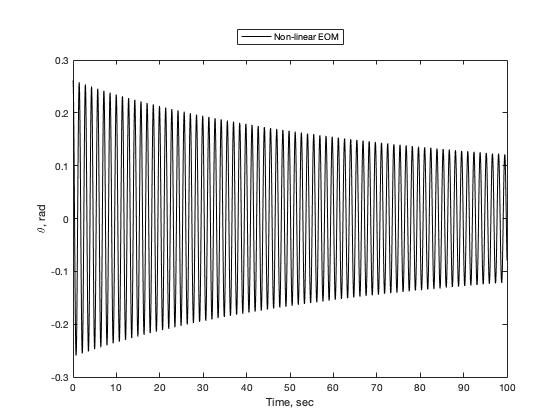
\includegraphics [width=5in,center]{PendulumThorne_01.jpg}

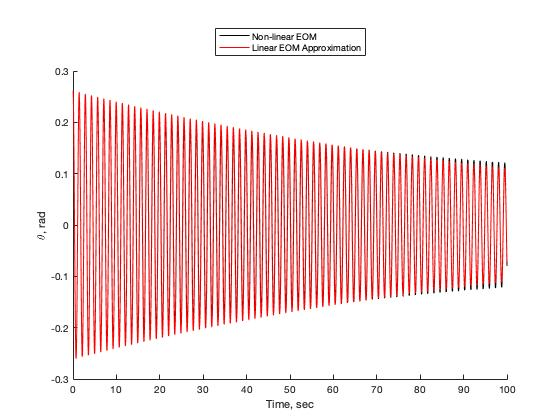
\includegraphics [width=5in,center]{PendulumThorne_02.jpg}

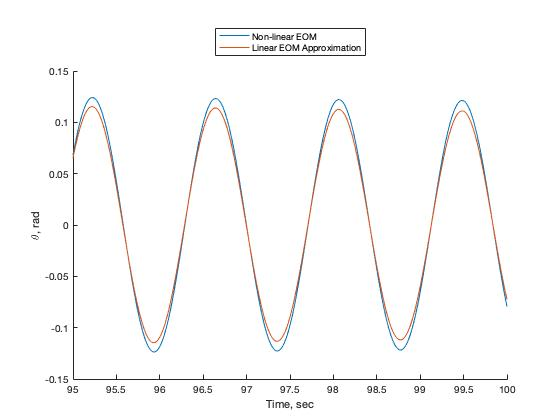
\includegraphics [width=5in,center]{PendulumThorne_03.jpg}
